\documentclass[10pt,conference]{IEEEtran}

\usepackage[T1]{fontenc}
\usepackage{cite}
\usepackage{amsmath,amssymb}
\usepackage{graphicx}
\usepackage{booktabs}
\usepackage{multirow}
\usepackage{array}
\usepackage{tabularx}
\usepackage[table]{xcolor}
\usepackage{url}
\usepackage{listings}
\usepackage{xspace}
\usepackage{tikz}

\lstset{
  basicstyle=\fontfamily{lmtt}\selectfont\footnotesize,
  keywordstyle=\mdseries,
  commentstyle=\mdseries,
  stringstyle=\mdseries,
  identifierstyle=\mdseries,
  columns=fullflexible,
  breaklines=true,
  frame=single,
  xleftmargin=0.5em,
  xrightmargin=0.5em
}

\newcommand{\tool}{\textsc{PyCGuard}\xspace}
\newcommand{\so}{safety obligation}
\newcommand{\sos}{safety obligations}
\newcommand{\dc}{discharge condition}
\newcommand{\dcs}{discharge conditions}
\newcommand{\code}[1]{{\fontfamily{lmtt}\selectfont\detokenize{#1}}}
% Abstract for: Finding Bugs in Python Native Extensions via Safety Obligation Checking
\newcommand{\paperabstract}{%
Python native extensions written in C/C++ are widely used to provide computational acceleration, hardware interaction, and system-level functionality for performance-critical Python libraries. Developing such extensions requires complying with the safety requirements of the Python/C API, including reference ownership management, null-value handling, exception propagation, and resource lifecycle management. However, these requirements are dispersed throughout extensive CPython documentation and are difficult to reason about across complex execution paths, causing bugs such as memory leaks, use-after-free vulnerabilities, and interpreter crashes that often elude conventional static analysis. We make the key observation that Python/C API safety requirements can be systematically modeled as \emph{dischargeable safety obligations}.
Based on a systematic study of CPython documentation and hundreds of real-world bugs, we derive 13 obligation categories that capture the dominant classes of Python/C API misuse and formally define the conditions under which each obligation is discharged.
We propose \tool, a bug detection framework for Python native extensions based on safety-obligation checking. \tool first employs lightweight static analysis to identify obligation-generating API usages and eliminate candidates lacking evidence of violations.
It then leverages an LLM to perform path-sensitive reasoning over obligation creation and discharge, determining whether the corresponding discharge conditions hold on every execution path. We evaluate \tool on 9 widely used open-source projects. \tool finds 86 previously unknown bugs with 82.7\% precision, of which 45 have been confirmed or fixed by maintainers.%
}


\title{Finding Bugs in Python Native Extensions via Safety Obligation Checking}

% ICSE 2027 Research Track uses double-anonymous review.
% Keep author information omitted for submission.
\author{}

\begin{document}

\maketitle

\begin{abstract}
\paperabstract
\end{abstract}

\begin{IEEEkeywords}
Python native extensions, Python/C API, static analysis, large language models, bug finding
\end{IEEEkeywords}

\section{Introduction}
\label{sec:introduction}

Python native extensions connect Python programs to C and C++ code. This
mechanism supports numerical kernels, device runtimes, operating-system
interfaces, and other functionality that cannot be implemented efficiently in
pure Python. The same boundary removes native code from the memory and error
management provided by the interpreter. Extension developers must instead
follow the Python/C API rules for reference ownership, nullable returns,
exception state, allocator domains, buffers, garbage collection, and thread
state \cite{pythoncapi,hu2020pythoncapi}. A violation can leak an object, access
a released value, corrupt interpreter state, or terminate the process that
hosts the extension.

These rules are difficult to enforce for two reasons. First, the relevant
information is distributed across the Python/C API reference manual. The
correct action depends on details such as whether an API returns a new or
borrowed reference, steals an argument, preserves an exception, or pairs with
a specific release operation. Second, compliance is path-sensitive. A newly
created object can be returned on one path, transferred to a container on a
second path, and require an explicit decrement on every remaining path. A
cleanup label that is correct for an owned reference can release a borrowed
reference on another branch. The defect is therefore not characterized by an
isolated call or a fixed API pair.

Prior Python/C analyzers make important progress on reference-count errors.
Pungi transforms reference-count behavior into affine programs
\cite{pungi2014}, while PyRefcon tracks both reference counts and object
lifecycle states with symbolic execution \cite{pyrefcon2023}. These analyses
target reference management and require detailed models of API and program
behavior. They do not provide a common representation for the broader set of
Python/C API requirements, including error-state discipline, allocator
agreement, buffer lifetime, numeric conversion, garbage-collection protocols,
and capsule metadata. General native-code analyzers cover some low-level
defects but lack the ownership and interpreter-state semantics that determine
whether a Python/C API use is correct.

Large language models offer a complementary ability to reason about source
code and natural-language specifications. Unconstrained bug finding, however,
asks a model to infer the relevant property, identify the program object, trace
the paths, and judge the violation in one step. This formulation makes reports
difficult to audit and exposes the result to unsupported bug hypotheses.
Recent hybrid systems improve practical static analysis with model reasoning
\cite{li2024llmstatic}, and specification-guided systems decompose external
requirements before checking code \cite{safe4u2025,rfcaudit2025}. The open
question for Python native extensions is how to formulate the API-specific
checking task so that static analysis and model reasoning have separate,
auditable roles. Unlike a typestate checker, \tool does not build a complete
transfer function for the whole program; unlike a pattern-based checker,
obligation definitions are separated from syntactic suspicion; and unlike
unconstrained LLM bug finding, the model is constrained to a fixed
API-induced property with enumerated safe alternatives.

We make the observation that a Python/C API requirement can be represented as
a \emph{safety obligation} together with explicit \emph{discharge
conditions}. An API use creates an obligation for a program object or runtime
state. The obligation is safe only when every relevant path satisfies an
admissible discharge condition. For example, a new reference satisfies its
ownership obligation when the path releases it, transfers it to an API that
steals ownership, or returns it to the caller. This representation states what
must hold without prescribing one program-analysis technique.

Based on this observation, we develop \tool. An offline construction process
extracts normative requirements and correct usage alternatives from CPython
documentation and real bug cases. The resulting specification contains 13
obligation categories and 41 discharge conditions. At detection time,
lightweight static analysis finds Python/C API call sites, binds them to
obligations, and collects the associated program objects. Fifteen syntactic
patterns implemented by the static analyzer prune obligation instances that
lack a suspicious shape. These patterns decide which obligation instances reach
the LLM, trading recall risk for cost reduction; they are not part of the
obligation semantics. For each retained instance, a large language
model receives the enclosing function, the obligation, and its discharge conditions.
The model identifies the trigger, enumerates relevant exits, checks each
condition, and returns a structured verdict and evidence.

We evaluate \tool through three research questions. The in-the-wild study
audits 104 high-confidence reports from widely used Python extension projects.
Eighty-six reports are real previously unknown defects, yielding 82.7\%
precision, and 45 findings were confirmed by project maintainers. The baseline
study reproduces PyRefcon and audits 80 deduplicated findings; it analyzes
why PyRefcon achieves only 7.5\% precision and examines the five
PyRefcon-only true positives to expose the boundary between Python/C API
obligations and generic C memory safety. Finally, the design study measures
the cost reduction from static pattern-based pruning and ablates the
chain-of-thought discharge step and the discharge-condition list to quantify
their individual contributions to bug recall.

This paper makes the following contributions:

\begin{itemize}
  \item We formulate Python/C API correctness as dischargeable safety
  obligations and construct a specification with 13 obligation categories
  and 41 discharge conditions.
  \item We design and implement \tool, which combines static obligation
  binding and pattern-based pruning with structured, path-oriented
  LLM checking and evidence-bearing reports.
  \item We evaluate \tool on real Python native extensions, find 86 previously
  unknown bugs at 82.7\% precision, compare with the closest reproducible
  analyzer, and isolate the effects of pruning and structured checking.
\end{itemize}

\section{Background and Motivation}
\label{sec:background}

\subsection{Python Native Extensions}

CPython exposes a C interface for defining modules, types, and functions and
for manipulating interpreter objects. A native function commonly parses
Python arguments, creates or accesses \code{PyObject} values, calls other
Python/C APIs, and returns either a Python object or an error indicator. The
interface uses conventions rather than a C type system to encode many safety
properties. A \emph{new reference} transfers ownership to the caller, while a
\emph{borrowed reference} remains owned elsewhere. Some APIs steal ownership
of an argument. Most object-producing APIs return \code{NULL} on failure and
set the thread-local exception indicator. Other APIs use integer sentinels,
and several resource APIs require a matching release operation
\cite{pythoncapi}.

The conventions interact. If \code{PyTuple_New} returns \code{NULL}, native
code must avoid dereferencing the result, preserve the pending exception, and
release objects acquired earlier on that path. If \code{PyTuple_SetItem}
succeeds, it steals an item reference, so a later decrement can access a freed
object. Correctness therefore depends on the API contract, the program object
to which the contract applies, and the path between acquisition and exit.

\subsection{Python/C API Safety Requirements}

We call a requirement \emph{API-induced} when a Python/C API call or a
Python-runtime callback creates the relevant duty. Reference ownership is the
most visible example, but the same structure appears in other parts of the
interface. A successful \code{PyObject\_GetBuffer} call creates a duty to call
\code{PyBuffer\_Release}; a fallible conversion creates a duty to check its
sentinel before use; releasing the global interpreter lock creates a duty to
reacquire it before another Python/C API call; and a garbage-collected type
creates a multi-part lifecycle duty for allocation, tracking, traversal,
clearing, and deallocation.

Three properties make these requirements unsuitable for simple call-pair
matching. A requirement can admit several correct outcomes, such as release,
transfer, or return. The appropriate outcome can differ across paths. In
addition, a syntactically present action can be semantically wrong, as when a
cleanup block decrements a borrowed reference or frees memory with an
allocator from another domain. These properties motivate an explicit
representation of both the duty and its admissible discharge conditions.

\subsection{Motivating Example}

Figure~\ref{fig:motivation} presents a defect found in the SciPy
\code{fitpack\_sphere} wrapper. The function receives \code{tt} and \code{tp}
from \code{PyArg\_ParseTuple}. When \code{iopt == -1}, it assigns these
borrowed references to \code{ap\_tt} and \code{ap\_tp}. A later validation
failure reaches the shared cleanup block, which decrements both variables.
The cleanup is correct when \code{iopt == 0} because that branch creates new
arrays, but it is unsafe for the borrowed-reference branch. The decrement can
prematurely release an object still owned by the caller.

\begin{figure}[t]
\begin{lstlisting}[language=C,numbers=left,firstnumber=1]
if (iopt == -1) {
    ap_tt = tt;                 // borrowed
    ap_tp = tp;                 // borrowed
} else if (iopt == 0) {
    ap_tt = PyArray_SimpleNew(...); // new
    if (ap_tt == NULL) goto fail;
    ap_tp = PyArray_SimpleNew(...); // new
    if (ap_tp == NULL) goto fail;
}
if (invalid_dimensions) goto fail;
...
fail:
Py_XDECREF(ap_tt);
Py_XDECREF(ap_tp);
return NULL;
\end{lstlisting}
\caption{Path-dependent ownership in \code{fitpack\_sphere}. The cleanup
releases owned arrays created by the second branch but also releases borrowed
arrays assigned by the first branch.}
\label{fig:motivation}
\end{figure}

A source-level pattern such as ``assignment followed by decrement'' cannot
distinguish the branches. Tracking only the final reference-count delta is
also insufficient unless the analysis recovers the ownership semantics of
both assignments and the feasibility of each cleanup path. Under our
formulation, the two assignments bind a reference-ownership obligation. The
new-reference branch is discharged by cleanup on failure and ownership
transfer on success. The borrowed-reference branch has no owned reference to
release, and the decrement violates the post-acquisition condition. The
example illustrates why the checker must combine API semantics with
path-specific discharge reasoning.

\section{Safety Obligation Construction}
\label{sec:construction}

\subsection{Overview}

The purpose of obligation construction is to turn dispersed API prose and bug
evidence into a reusable checking specification. Construction occurs offline
and is independent of a target project. Each specification entry records a
trigger, the safety property induced by the trigger, the program subject, and
the conditions that discharge the property. Detection then instantiates these
entries at concrete API calls, as described in
Section~\ref{sec:pipeline}.

The specification contains only semantic information: a safety obligation and
the conditions that discharge it. Operational optimizations are deliberately
kept outside this representation. For example, the absence of a nearby
\code{Py\_DECREF} cannot define an ownership violation because the reference
may instead be transferred or returned. Section~\ref{sec:pipeline} introduces
such syntactic patterns as part of static pruning.

\subsection{Evidence Sources}

The primary source is the CPython 3.14 Python/C API reference manual
\cite{pythoncapi}. We inspect chapters that specify object ownership,
reference counting, exception handling, memory allocation, buffer access,
thread state, garbage-collection support, container iteration, argument
conversion, and capsules. Normative statements identify the trigger and the
required property. Notes and examples provide admissible safe outcomes. We
also inspect real Python/C API bug-fix commits. We mined 442 fix commits
from 23 open-source Python extension repositories via the GitHub API,
filtering to commits that modify C or C++ source files and whose messages or
diffs reference Python/C API constructs; 395 of the 442 commits involve
CPython FFI code. These cases expose requirements that are easy to overlook in
documentation, interactions between obligations, and recurring code forms
suitable for pruning patterns. We stopped adding obligation categories after
three consecutive documentation sections and ten consecutive bug cases
introduced no new obligation type. The empirical studies by Yang and Cai and
by Hu and Zhang provide independent corroboration that ownership, exception,
and compatibility mistakes are the dominant failure classes in real-world
cross-language code \cite{yang2025dissecting,hu2020pythoncapi}.

We use bug cases to refine and validate documented requirements, not to infer
correctness from frequency. A recurring idiom is not considered safe when it
contradicts the API documentation. Conversely, an unusual idiom can discharge
an obligation when its path and ownership semantics satisfy the documented
property.

\subsection{Construction Procedure}

The construction procedure has three steps. First, we extract a candidate
requirement and record its triggering APIs, subject, failure mode, and cited
documentation. For the reference-counting rule that a new reference belongs
to its caller, for example, the trigger is a new-reference-returning API, the
subject is its result, and the failure modes include leaks and premature
release.

Second, we normalize requirements by the safety property rather than by API
name. APIs that create the same duty share one obligation even when their
surface signatures differ. Requirements remain separate when they require
different evidence. Reference ownership and null validation can therefore be
bound to the same call without collapsing their meanings.

Third, we derive discharge conditions from documented safe alternatives and
validated fixes. Conditions are intentionally sufficient rather than
exhaustive. An owned reference, for example, can be released on every exit,
transferred to an ownership-consuming API, or returned to the caller. A
condition records the semantic outcome, not one exact syntax. We merge
conditions that establish the same outcome and retain separate conditions
when they require different reasoning.

\subsection{Safety Obligations}

Table~\ref{tab:obligations} summarizes the resulting specification. The 13
categories cover reference lifecycle, failure handling, native resources,
type and value agreement, and runtime protocols. A single API can bind several
categories. For example, an object-producing call can create ownership,
null-validation, cleanup, and exception-state obligations. Conversely, one
category can cover many APIs that share a contract.

\begin{table*}[t]
\caption{Python/C API safety obligation types and their discharge conditions.}
\label{tab:obligations}
\centering
\fontsize{6.2}{6.7}\selectfont
\setlength{\tabcolsep}{2.1pt}
\renewcommand{\arraystretch}{1.08}
\begin{tabularx}{\textwidth}{|>{\centering\bfseries\arraybackslash}p{2.2cm}|>{\centering\arraybackslash}p{6.5cm}|>{\centering\bfseries\arraybackslash}p{3.1cm}|X|}
\hline
\rowcolor{black!10}
\rule{0pt}{2.4ex}\textbf{Obligation type} & \textbf{Obligation description} & \textbf{Discharge condition} & \multicolumn{1}{c|}{\textbf{Discharge-condition description}} \\
\hline
\multirow[c]{4}{=}{\centering Reference ownership} &
\multirow[c]{4}{=}{\centering Resolve every owned reference and prevent reuse after ownership transfer.} &
Explicit release & Release the reference on every exit path. \\
\cline{3-4}
& & Ownership transfer & Pass it to an API that assumes release responsibility. \\
\cline{3-4}
& & Return to caller & Return it as the function's new-reference result. \\
\cline{3-4}
& & Post-steal non-use & Do not use or release it after a steal unless first retained. \\
\hline
\multirow[c]{2}{=}{\centering Reference validity} &
\multirow[c]{2}{=}{\centering Keep a borrowed reference valid at every use.} &
Scope-safe use & Finish all uses before any operation that can invalidate it. \\
\cline{3-4}
& & Strong promotion & Retain it before invalidation or persistent storage. \\
\hline
\multirow[c]{3}{=}{\centering Null/error validation} &
\multirow[c]{3}{=}{\centering Prove a fallible result valid before unsafe use.} &
Dominating check & Check NULL or the error sentinel before every unsafe use. \\
\cline{3-4}
& & Infallible source & Obtain the value from a source infallible for this input. \\
\cline{3-4}
& & NULL-safe use & Use the value only in NULL-tolerant operations. \\
\hline
\multirow[c]{4}{=}{\centering Error propagation} &
\multirow[c]{4}{=}{\centering Handle or propagate failures and clean resources on failing paths.} &
Cleanup block & Release acquired resources and return an error indicator. \\
\cline{3-4}
& & Early return & Release resources inline before returning the error. \\
\cline{3-4}
& & Recovery & Clear the exception and execute an intentional fallback. \\
\cline{3-4}
& & NULL-safe cleanup & Initialize cleanup variables and use NULL-safe releases. \\
\hline
\multirow[c]{4}{=}{\centering Exception state} &
\multirow[c]{4}{=}{\centering Resolve pending exceptions before normal API work and preserve prior state.} &
Immediate check & Inspect exception state before a non-safe API call. \\
\cline{3-4}
& & Safe-only work & Perform only exception-safe operations while one is pending. \\
\cline{3-4}
& & Prompt resolution & Clear and recover, or return an error, before normal work. \\
\cline{3-4}
& & Dealloc preservation & Save and restore pre-existing state around finalization. \\
\hline
\multirow[c]{4}{=}{\centering Resource protocol} &
\multirow[c]{4}{=}{\centering Pair each acquisition with its correct release and allocator domain.} &
Matched release & Apply the matching release on every successful-acquire path. \\
\cline{3-4}
& & Domain consistency & Free memory through the allocator domain that created it. \\
\cline{3-4}
& & Failure-aware skip & Skip release when acquisition failed and returned NULL. \\
\cline{3-4}
& & Safe reallocation & Preserve the original pointer until reallocation succeeds. \\
\hline
\multirow[c]{5}{=}{\centering Post-release safety} &
\multirow[c]{5}{=}{\centering Prevent repeated release, later access, and reentrant inconsistent state.} &
NULL assignment & Clear the pointer immediately after releasing it. \\
\cline{3-4}
& & No later access & Do not read, dereference, or pass the released resource. \\
\cline{3-4}
& & Container-safe update & Use Py\_CLEAR or Py\_SETREF for observable members. \\
\cline{3-4}
& & Local-only scope & Ensure reentrant code cannot observe the released object. \\
\cline{3-4}
& & Buffer-alias lifetime & Finish alias reads before releasing the underlying buffer. \\
\hline
\multirow[c]{2}{=}{\centering Type agreement} &
\multirow[c]{2}{=}{\centering Match API formats with C types, widths, encodings, and protocols.} &
Format-type match & Match each format code to the corresponding C argument type. \\
\cline{3-4}
& & Platform width & Use format codes consistent with platform-dependent widths. \\
\hline
\multirow[c]{3}{=}{\centering Numeric and bounds safety} &
\multirow[c]{3}{=}{\centering Prevent narrowing, allocation overflow, and out-of-bounds access.} &
Range check & Check the range before narrowing or indexed access. \\
\cline{3-4}
& & Allocation check & Check size arithmetic for overflow before allocation. \\
\cline{3-4}
& & Sufficient type & Store the value in a type wide enough for the platform. \\
\hline
\multirow[c]{2}{=}{\centering Thread safety} &
\multirow[c]{2}{=}{\centering Use the Python/C API under a valid interpreter-lock context.} &
Valid context & Hold the GIL whenever invoking the Python/C API. \\
\cline{3-4}
& & Blocking-I/O release & Release the GIL for blocking work and reacquire it first. \\
\hline
\multirow[c]{3}{=}{\centering GC lifecycle} &
\multirow[c]{3}{=}{\centering Complete allocation, tracking, traversal, clearing, and deallocation.} &
GC allocation domain & Use matching GC-aware allocation and deallocation. \\
\cline{3-4}
& & Tracking protocol & Track after initialization and untrack before field clearing. \\
\cline{3-4}
& & Traverse and clear & Visit every owned field and clear it with Py\_CLEAR. \\
\hline
\multirow[c]{2}{=}{\centering Iteration integrity} &
\multirow[c]{2}{=}{\centering Do not structurally mutate a container during iteration.} &
Read-only body & Perform no direct or indirect mutation while iterating. \\
\cline{3-4}
& & Iteration copy & Iterate over a copy when the original may be mutated. \\
\hline
\multirow[c]{3}{=}{\centering Capsule name stability} &
\multirow[c]{3}{=}{\centering Keep a capsule name valid and consistent throughout its lifetime.} &
String literal & Use an immutable string literal with static lifetime. \\
\cline{3-4}
& & Static storage & Store the name in a static or module-lifetime constant. \\
\cline{3-4}
& & Destructor-managed & Free a dynamic name only in the capsule destructor. \\
\hline
\end{tabularx}
\end{table*}

\subsection{Discharge Conditions}

Let $o$ be an obligation instance bound in function $f$, let $D(o)$ be its
discharge conditions, and let $\Pi(o,f)$ be the relevant paths from its trigger
to an exit or unsafe use. For the default disjunctive mode, the intended
judgment is
\begin{equation}
  \mathit{Safe}(o,f) \equiv
  \forall \pi \in \Pi(o,f),\; \exists d \in D(o): d(\pi).
  \label{eq:discharge}
\end{equation}
Thus, different paths can satisfy different conditions. SO-11 uses a
conjunctive mode because allocation, tracking, traversal, clearing, and
deallocation are complementary aspects of one garbage-collection protocol.
For this category, all applicable conditions must hold.

Equation~\ref{eq:discharge} defines the question asked by the checker. It does
not claim that the LLM enumerates paths soundly or proves the equation. The
structured output records the paths and condition judgments used to reach a
verdict so that a reviewer can inspect the reasoning.

The ownership obligation in Figure~\ref{fig:motivation} has four conditions:
explicit release, ownership transfer, return to the caller, and no use after a
steal. On each failure path of the new-reference branch, explicit release
holds. On the successful branch, returned arrays transfer ownership. The
borrowed-reference branch does not create an owned reference, so its cleanup
must not apply the release action. Binding ownership semantics to the concrete
assignment exposes this mismatch.

The same representation applies beyond ownership. Null validation can be
discharged by a dominating check, an infallible source for the given input, or
exclusively null-tolerant uses. A resource protocol requires matched release,
allocator-domain agreement, and a failure-safe reallocation pattern. Capsule
names can use literal, static, or destructor-managed storage. These conditions
specify semantic outcomes rather than one cleanup-label name, macro, or branch
shape, allowing equivalent C, C++, and generated-wrapper idioms.

\subsection{Traceability and Evolution}

Each obligation entry retains its trigger API categories, discharge
conditions, and documentation locations in one versioned JSON record. This
structure supports two audits. A specification audit can trace a
property or condition back to the CPython reference chapter that motivates it.
A detection audit can trace a report from a concrete call site to the bound SO,
the evaluated DCs, and the final path evidence. Keeping both links is necessary
because a correct API rule can still be bound to the wrong subject, and a
correct binding can still receive an incorrect path judgment.

The specification is designed to evolve with CPython. A new API that follows
an existing ownership or error convention usually adds a trigger without
creating a new SO. A new semantic requirement adds a condition or category
only when the existing vocabulary cannot express its safe outcomes. Static
pruning patterns are versioned separately in the analyzer, so refining a
heuristic does not change the meaning of past obligations.

\section{Detection Pipeline}
\label{sec:pipeline}

\subsection{Overview}

Figure~\ref{fig:overview} presents the two phases of \tool. The offline phase
constructs the obligation specification described in
Section~\ref{sec:construction}. The online phase consumes a native-extension
project and produces auditable bug reports. Static analysis first discovers
candidate functions, binds API calls to obligations, and prunes obligation
instances using syntactic patterns. Structured LLM checking then
tests every retained obligation against its discharge conditions. Only
high-confidence violated judgments become reports.

\begin{figure*}[t]
\centering
\begin{tikzpicture}
  \node[anchor=south west,inner sep=0] (overview) at (0,0) {
    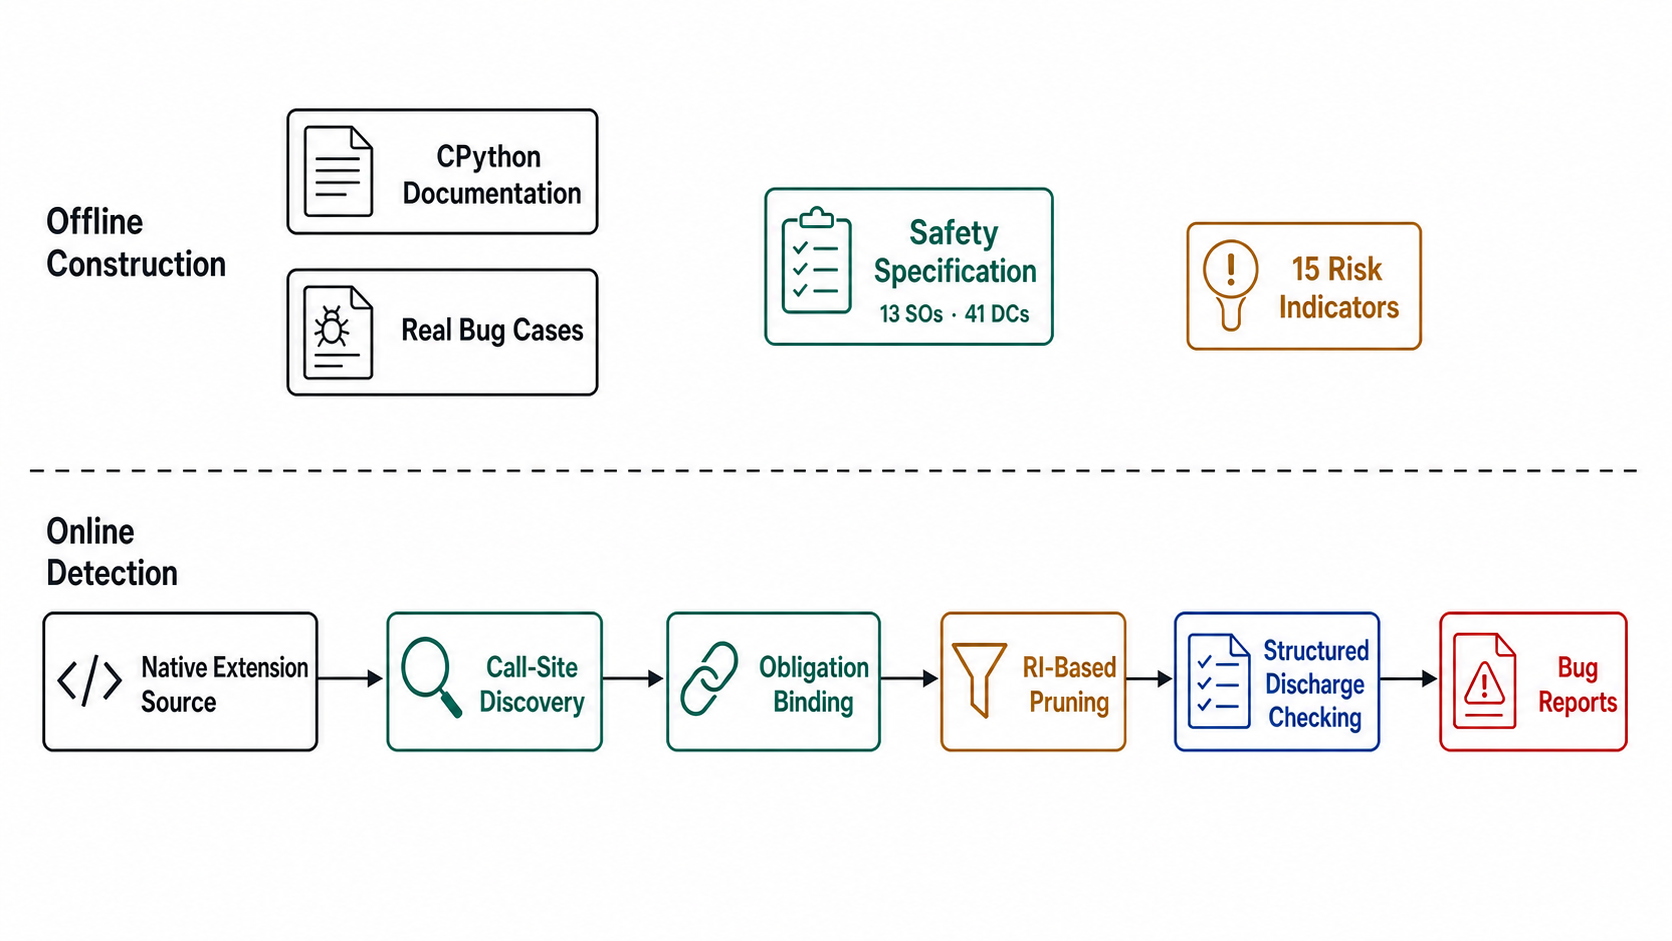
\includegraphics[width=0.90\textwidth]{figures/pycguard_overview.png}
  };
  \begin{scope}[x={(overview.south east)},y={(overview.north west)}]
    \tikzset{flow/.style={->,>=stealth,line width=0.55pt,draw=black!80,
                          rounded corners=1pt}}
    % Evidence sources to offline artifacts.
    \draw[flow] (0.355,0.82) -| (0.455,0.72);
    \draw[flow] (0.355,0.64) -| (0.455,0.68);
    % Static pruning owns these patterns; mask the obsolete offline RI box.
    \fill[white] (0.70,0.60) rectangle (0.87,0.80);
    % Offline artifacts to their only online consumers.
    \draw[flow] (0.505,0.61) -- (0.505,0.40) -- (0.465,0.40)
                -- (0.465,0.33);
    \draw[flow] (0.590,0.61) -- (0.590,0.39) -- (0.765,0.39)
                -- (0.765,0.33);
  \end{scope}
\end{tikzpicture}
\caption{PyCGuard workflow. Safety obligations and discharge conditions define
the checked properties. Static pattern matching prunes bound instances before
LLM checking.}
\label{fig:overview}
\end{figure*}

The pipeline uses the function as its context unit and a pair $(f,o)$ as its
checking unit. Grouping calls by function preserves cleanup labels and branch
conditions shared by several API calls. Separating obligations prevents one
large prompt from asking the model to discover arbitrary defects. A function
can therefore produce several checking units before pruning, each with one
property and a small set of discharge alternatives.

\subsection{Candidate Generation}

\paragraph{Source discovery.}
The scanner walks C and C++ source and header files. A file is selected when it
directly includes \code{Python.h} or contains Python/C API symbols. The second
criterion covers indirect includes and generated wrappers. Header files are
recorded because inline extension code can reside in headers, although the
evaluation reports source-file coverage separately.

\paragraph{Call-site discovery.}
Tree-sitter parses each selected file and identifies call expressions and their
enclosing function definitions. The current specification indexes 147 API
names. Calls outside a function are ignored because the checker requires an
enclosing control-flow context. Parse errors are retained as metadata so that
malformed or dialect-specific input can be audited.

\paragraph{Obligation binding.}
For each indexed call, \tool retrieves all associated SOs and records the API,
arguments, location, and obligation category. It extracts the subject from the
left-hand side for object-producing APIs, from the consumed argument for
steal-reference APIs, and from the first argument for decrement operations.
All trigger sites in the same function are aggregated. Repeated calls at the
same location are deduplicated, and the union of bound SOs forms the unpruned
candidate.

\paragraph{Local use facts.}
The analyzer traverses the enclosing syntax tree for references to each
trigger variable. It classifies simple assignments, null checks, decrement
calls, ownership-consuming calls, returns, and other uses. It also follows
simple local aliases. These facts support static pattern matching; they are not
used to establish a final safe verdict.

\subsection{Static Pattern-Based Pruning}

The pruning module defines 15 risk-indicator patterns for eight SO categories;
they are analyzer rules rather than fields in the obligation specification.
The module maintains a registry from an SO identifier to an executable pattern
checker. Each checker consumes the trigger sites, the local-use facts collected
for trigger variables, and the enclosing function text. This organization
keeps pattern evolution independent of the JSON specification: adding or
weakening a screen changes candidate selection but not the property sent to the
LLM.

The patterns fall into three operational groups. Ownership and lifetime
patterns look for a new reference without a release, transfer, or return; an
inline new-reference result that cannot be discharged later; borrowed-reference
use; repeated release sites; uninitialized cleanup variables; and mutation of
a reused tuple. Validation and error-state patterns detect a nullable result
whose first classified use is not a check, a callback without an exception
check, tri-state APIs treated as booleans, and APIs that suppress exceptions.
Resource and representation patterns cover unmatched allocation/release
operations, unchecked typed casts, missing write-back resolution, and narrowing
conversions. These are deliberately syntactic approximations. A matched pattern
retains an SO for checking; it never establishes a violation or replaces a DC.

For ownership, for example, the screen retains a new reference when it cannot
find a release, transfer, or return form. For null validation, it retains a
result when the first classified use after creation is not a null check. The
subsequent LLM prompt contains the SO and complete DC set, but not a claim that
the matched pattern is defective. The checker must still reason about all
relevant paths and admissible discharge alternatives.

The screen is intentionally conservative in two ways. An SO without an
implemented indicator is retained. If screening removes every SO bound to a
function, the implementation restores the original set rather than dropping
the function. This fallback prevents a candidate from disappearing solely
because the current pattern vocabulary does not describe it, although it also
limits the maximum reduction. RQ3 measures the actual reduction and checks
whether any known defect loses its $(f,o)$ pair.

\subsection{Structured Discharge Checking}

For every retained pair, the checker constructs a prompt with four components:
the SO description, its check mode, the complete DC list, and the full
enclosing function. We use the full function because exits, cleanup labels,
and ownership transfers often lie outside a local statement slice. Line
numbers, trigger sites, and variables from static analysis orient the model,
but the model must justify its decision using source evidence.

The requested procedure mirrors Equation~\ref{eq:discharge}. The model first
identifies the triggering call and subject. It then enumerates normal returns,
early returns, error jumps, and other relevant exits. For each path, it records
whether each applicable DC holds and cites variables and lines. A disjunctive
obligation is \code{SAFE} only when every listed path has at least one
satisfied DC. A conjunctive obligation requires every applicable aspect. If a
path lacks a discharge, the verdict is \code{VIOLATED} and the output names the
path and failed conditions.

The response schema contains the trigger API, subject, path list, per-condition
judgments, verdict, violation detail, and confidence. The JSON structure makes
missing paths and unsupported condition claims visible during audit. It does
not eliminate model error, which we evaluate through manual review, malformed
output, prompt ablation, and cross-model agreement.

\paragraph{Multiple triggers and exits.}
A function can contain several calls that bind the same SO. The prompt retains
all trigger sites and asks the model to identify the subject of each relevant
instance. This matters when a cleanup block releases several partially
initialized objects or when the same nullable API appears in separate
branches. The path record must connect a trigger and subject to the discharge
evidence; a decrement of another variable does not satisfy the condition.
Normal returns, error returns, cleanup jumps, and fall-through exits are all
within scope. The checker does not treat syntactic reachability as proof that a
path is feasible.

\paragraph{Check ordering.}
Retained SO identifiers are sorted before model calls. Stable ordering makes
runs easier to compare and gives the early-stop policy deterministic semantics
for a fixed model response. Early stop means that the tool reports at most the
first violated SO checked for one function in a run. The evaluation therefore
counts report units rather than claiming to enumerate every defect effect in a
function. Disabling early stop is supported for diagnostic runs that need all
SO judgments.

\paragraph{Response validation.}
The checker accepts only \code{SAFE} and \code{VIOLATED} verdicts in the
expected JSON object. Network failures are retried with increasing delays.
JSON recovery removes limited trailing-comma errors and can recover an explicit
verdict from otherwise malformed text; all other responses remain unknown.
Recovery status and raw text are preserved so that a parsed verdict does not
hide format noncompliance. RQ3 reports malformed and unknown rates separately
from detection quality.

\subsection{Report Generation}

The default checker stops after the first violated SO in a function. This
early-stop policy bounds repeated model calls and gives each report one primary
property. Report generation suppresses safe judgments, malformed outputs, and
violations below high confidence. A retained report identifies the project,
file, function, SO, trigger location, subject, violation path, and model
evidence. The high-confidence filter defines the RQ1 audit population; it does
not imply that medium- or low-confidence outputs are false.

\subsection{Implementation}

\tool is implemented in Python. The static analysis frontend uses the
Tree-sitter C and C++ grammars for parsing and AST-based pattern matching.
The obligation specification is stored as JSON, from which the tool builds
the API index and prompt fragments at load time. The pruning stage applies
AST pattern queries to filter obligation instances before any LLM call.
The LLM backend is \code{claude-sonnet-4} at temperature 0.

\section{Evaluation}
\label{sec:evaluation}

\subsection{Research Questions}

We organize the evaluation around three questions:

\begin{description}
  \item[RQ1:] How effectively does \tool find previously unknown bugs in real
  Python native extensions?
  \item[RQ2:] How does \tool compare with existing Python native-extension bug
  detectors, and why does it miss bugs found by another detector?
  \item[RQ3:] How do static pattern-based pruning and structured prompt
  design affect the cost and bug recall of \tool?
\end{description}

RQ1 evaluates the end-to-end result after the high-confidence filter. RQ2
compares with the closest reproducible analyzer and studies non-overlapping
defects. RQ3 isolates the two design decisions that control analysis cost and
model behavior.

\subsection{Subjects and Protocol}

We selected nine open-source projects according to three criteria:
(1) the project implements substantial performance-critical or system-facing
functionality in C or C++; (2) the project is actively maintained with a
public issue tracker; and (3) the project is widely adopted, as reflected
by GitHub star count and PyPI download volume. Table~\ref{tab:subjects} reports the quantitative
corpus. The scanner manifest contains 489 C/C++ source files from these
projects.

\begin{table}[t]
\caption{Subjects and manually audited high-confidence PyCGuard reports.}
\label{tab:subjects}
\centering
\small
\setlength{\tabcolsep}{3.5pt}
\begin{tabular}{l|r|r|r|r|r}
\toprule
Project & Stars & Bug Reports & TP & FP & Precision \\
\midrule
SciPy      & 14.8k & 24 & 20 & 4 & 83.3\% \\
pandas     & 49.1k & 18 & 15 & 3 & 83.3\% \\
NumPy      & 32.3k & 15 & 13 & 2 & 86.7\% \\
Pillow     & 13.6k & 15 & 13 & 2 & 86.7\% \\
PyTorch    & 101k  & 12 & 10 & 2 & 83.3\% \\
PycURL     &  1.2k &  7 &  5 & 2 & 71.4\% \\
ujson      &  4.5k &  6 &  5 & 1 & 83.3\% \\
TensorFlow & 196k  &  4 &  3 & 1 & 75.0\% \\
psutil     & 11.2k &  3 &  2 & 1 & 66.7\% \\
\midrule
Total      &       & 104 & 86 & 18 & 82.7\% \\
\bottomrule
\end{tabular}
\end{table}

\paragraph{PyCGuard configuration.}
RQ1 uses the configuration in Section~\ref{sec:pipeline}, including
\code{claude-sonnet-4}, temperature 0, early stop, and the
high-confidence report filter. The analysis unit is one project, file,
function, and SO tuple. Several unsafe effects in one tuple are counted as one
report. We do not use lower-confidence violations to calculate precision.
Medium- and low-confidence outputs are suppressed and not audited;
all precision claims in this paper are restricted to the 104
high-confidence reports.

\paragraph{Manual audit.}
For each report, we inspect the complete function, the reported path, the
Python/C API contract, and relevant callees or macros when needed. A report is
a true positive when the reported behavior violates the claimed SO on a
feasible path. A report is a false positive when the path is infeasible, a
hidden ownership or cleanup action discharges the SO, or the model
misinterprets the API contract. Precision is $TP/(TP+FP)$. Because the study
starts from tool reports rather than a complete defect oracle, we do not claim
recall for the in-the-wild corpus.

\paragraph{Baseline protocol.}
We run PyRefcon over all C/C++ source files accepted by its compilation
pipeline. We parse 224 HTML warnings and group warnings with the same project,
file, function, and bug type into 80 audit units. Each unit is inspected using
the reported trace and source context. This deduplication prevents repeated
paths for one defect from inflating the result.

\subsection{RQ1: In-the-Wild Bug Finding}

\tool reports 104 high-confidence findings. Manual audit identifies 86 true
positives and 18 false positives, for a precision of
$86/104=82.7\%$. The true positives cover a diverse range of defect
classes, including reference ownership errors, null dereferences,
exception-state violations, resource leaks, post-release safety errors,
type mismatches, and numeric bounds violations. This distribution
supports the central scope claim: Python native-extension defects extend
beyond reference-count imbalance.

The project-level result is not dominated by one code base. Seven projects
contribute at least five true positives, and all nine projects in the audited
corpus contain at least two. Of these findings, 45 were accepted by project
maintainers, of which 13 have been fixed and 32 are confirmed but awaiting
a patch.

The motivating defect in Figure~\ref{fig:motivation} illustrates a common
benefit of obligation checking. A shared cleanup block appears locally
responsible because it decrements every array variable. The ownership
obligation forces the checker to distinguish the borrowed and new-reference
branches. Similar true positives require relating a fallible allocation to a
later unsafe macro, preserving exception state across callbacks, or pairing a
buffer acquisition with all failure exits.

\paragraph{False positives.}
Table~\ref{tab:fp} categorizes the 18 false positives by their immediate root
cause. Six require precise knowledge of whether an API borrows, creates, or
steals a reference. The next largest group requires reasoning about complex
control flow. Macros, C++ destructors, and paired teardown functions hide
discharge evidence outside the source form given to the model. These failures
suggest that the dominant limitation is missing semantic context rather than a
lack of obligation categories.

\begin{table}[t]
\caption{Root causes of the 18 false-positive PyCGuard reports.}
\label{tab:fp}
\centering
\small
\begin{tabular}{lr}
\toprule
Root cause & Count \\
\midrule
Borrowed, new, or stolen reference semantics & 6 \\
Complex control flow & 3 \\
Macro expansion & 2 \\
C++ RAII or smart-pointer cleanup & 2 \\
Interprocedural cleanup & 2 \\
State-machine behavior & 1 \\
Standard error propagation & 1 \\
Infeasible retry path & 1 \\
\bottomrule
\end{tabular}
\end{table}

\subsection{RQ2: Comparison with Existing Tools}

PyRefcon is the closest reproducible detector because it directly analyzes
Python native code and models Python object lifecycle and reference counts
\cite{pyrefcon2023}. We run PyRefcon over all 489 C/C++ source files in
the nine projects and manually audit each deduplicated warning unit.
Table~\ref{tab:baseline} reports the per-project result.

\begin{table}[t]
\caption{PyRefcon per-project audit result on the nine subject projects.}
\label{tab:baseline}
\centering
\small
\begin{tabularx}{\columnwidth}{X|r|r|r|r|r}
\toprule
Project & Warnings & Units & TP & FP & Precision \\
\midrule
SciPy      & 76 & 11 &  1 & 10 & 9.1\%  \\
pandas     & 32 & 16 &  4 & 12 & 25.0\% \\
NumPy      & 34 & 14 &  1 & 13 & 7.1\%  \\
Pillow     & 34 & 17 &  0 & 17 & 0.0\%  \\
PyTorch    & \texttimes & \texttimes & \texttimes & \texttimes & \texttimes \\
PycURL     & 26 & 12 &  0 & 12 & 0.0\%  \\
ujson      &  6 &  3 &  0 &  3 & 0.0\%  \\
TensorFlow &  6 &  2 &  0 &  2 & 0.0\%  \\
psutil     & 10 &  5 &  0 &  5 & 0.0\%  \\
\midrule
Total      & 224 & 80 &  6 & 74 & 7.5\%  \\
\bottomrule
\end{tabularx}
\end{table}

PyRefcon emits 224 raw warnings across 38 of 489 target files; 151 of
the remaining files fail to compile in its analysis environment.
PyTorch fails entirely because its required CMake-generated headers
are absent from the standalone analysis toolchain.
After deduplication, 80 audit units remain, of which only 6 are true
positives (7.5\% precision).

The low true-positive count reflects a fundamental scope mismatch.
PyRefcon models only reference-count ownership, so it cannot represent
exception-state rules, resource-pairing obligations, type-agreement
requirements, numeric bounds, or post-release safety. These five categories
account for 35 of PyCGuard's 86 true positives and are entirely outside
PyRefcon's scope. Even within
reference counting, one of the six PyRefcon true positives overlaps a
PyCGuard finding; the remaining five are raw-pointer null dereferences
or generic \code{malloc}/\code{free} flows whose correctness depends on
project-local C invariants rather than a Python/C API contract, so
PyCGuard's static binder never creates an obligation for them.

The 74 false positives reveal the cost of modeling a single lifecycle
pattern without explicit discharge alternatives. Fifty-one reports trace
a standard \code{Py\_DECREF} call into the CPython deallocation body
and flag it as an ownership release error, treating any decrement as
suspect regardless of whether the preceding acquire-release pair is
balanced. Eight misread cleanup paths that explicitly destroy an
already-allocated object. Nine miss cross-function or cross-iteration
invariants, and six arise from macro expansion that hides the actual
reference semantics. These patterns are precisely the failure modes
that PyCGuard's discharge-condition list is designed to rule out: each
discharge condition represents a syntactic form that, when present on
every exit path, provides evidence that the obligation is satisfied without requiring
interprocedural or macro-expansion reasoning.

We attempted to run CpyChecker using the configuration reported by
PyRefcon. The plugin either disabled reference-count verification on
GCC 7 and later, failed to initialize with the matching Python headers,
or produced no plugin warnings in the usable configuration. We
therefore report it as unavailable. Pungi has no public implementation.
RID targets general reference-count inconsistencies on the Linux kernel
\cite{rid2016} and is not a direct Python/C baseline. CHARON analyzes
cross-language vulnerability flows \cite{charon2025} with no public
artifact for a same-project run. These tools are discussed qualitatively
and do not receive quantitative rows.

\subsection{RQ3: Design Analysis}

RQ3 quantifies the value of two design decisions that govern the
end-to-end behavior of \tool. The first is static pattern-based
pruning, which decides how many obligations reach the LLM. The second
is the obligation prompt, which decides how the LLM reasons about each
obligation that it does see. We measure pruning by its marginal effect
on checking cost over the 86 manually validated true-positive cases;
this controlled replay holds the analyzed function/SO set fixed and
therefore isolates the cost contribution of static pruning. We measure
the prompt by its effect on bug recall across the same 86 cases.

\paragraph{Cost effect of pruning.}
Table~\ref{tab:pruning-cost} reports per-project token usage, dollar
cost, and wall-clock time for a controlled replay of the 86 RQ1
true-positive cases with pruning disabled and enabled. The same
project/file/function/SO targets are used in both configurations;
differences in token usage and time are therefore attributable to
pruning rather than to different report populations. Cost uses
Anthropic's published Claude Sonnet 4 pricing
(\$3 / MTok input, \$15 / MTok output). The high-confidence filter and
the early-stop rule from Section~\ref{sec:pipeline} are kept enabled
in both configurations so that the comparison reflects only the
pruning step.

\begin{table*}[t]
\caption{Per-project LLM cost on the 86 true positives with and without static pruning.}
\label{tab:pruning-cost}
\centering
\small
\setlength{\tabcolsep}{4.5pt}
\begin{tabular}{l rrrr c rrrr c r}
\toprule
& \multicolumn{4}{c}{Without pruning} & & \multicolumn{4}{c}{With pruning} & & \\
\cmidrule{2-5} \cmidrule{7-10}
Project & Input (K) & Output (K) & Cost (\$) & Time (min) & &
          Input (K) & Output (K) & Cost (\$) & Time (min) & & Cost Reduction (\%) \\
\midrule
SciPy      & 103.0 & 24.7 & 0.68 & 8.0 & &  62.3 & 17.1 & 0.44 & 5.5 & & 35.3\% \\
pandas     &  28.4 & 13.8 & 0.29 & 4.4 & &  17.6 &  9.8 & 0.20 & 3.1 & & 31.0\% \\
NumPy      &  81.6 & 15.7 & 0.48 & 5.3 & &  47.5 & 10.4 & 0.30 & 3.5 & & 37.5\% \\
Pillow     &  37.9 & 15.0 & 0.34 & 4.8 & &  22.7 & 10.2 & 0.22 & 3.2 & & 35.3\% \\
PyTorch    &  15.5 &  8.4 & 0.17 & 2.7 & &  11.9 &  7.4 & 0.15 & 2.4 & & 11.8\% \\
PycURL     &  10.8 &  7.4 & 0.14 & 2.3 & &   6.0 &  4.6 & 0.09 & 1.4 & & 35.7\% \\
ujson      &   6.3 &  4.7 & 0.09 & 1.6 & &   4.1 &  3.5 & 0.06 & 1.2 & & 33.3\% \\
TensorFlow &   3.4 &  2.7 & 0.05 & 0.9 & &   2.4 &  2.2 & 0.04 & 0.7 & & 20.0\% \\
psutil     &   9.3 &  2.4 & 0.06 & 0.8 & &   4.8 &  1.4 & 0.04 & 0.4 & & 33.3\% \\
\midrule
Total      & 296.2 & 94.9 & 2.31 & 30.7 & & 179.2 & 66.7 & 1.54 & 21.5 & & 33.3\% \\
\bottomrule
\end{tabular}
\end{table*}

Processing the 86 true-positive cases with pruning disabled costs
\$2.31 and takes 30.7 minutes of wall-clock LLM time. Enabling
pruning cuts this to \$1.54 and 21.5 minutes, a reduction of 33.3\%
in cost and 30\% in time. The driver is a sharp drop at the
binding stage: pruning eliminates a substantial fraction of bound
obligations per project before any model call, so
the LLM never pays the per-call overhead for cases it would
ultimately answer SAFE. The end-to-end reduction is smaller than the
binding-stage reduction because the obligations that survive pruning
are harder on average; the model emits longer structured rationale on them,
which cost more output tokens per call. Pruning therefore
concentrates LLM effort on syntactically suspicious cases rather than
removing work uniformly.

Per-project savings track the fraction of callback-heavy and
allocator-only functions that the binders hit but pruning can
dismiss. SciPy, NumPy, PycURL, and psutil each achieve at least 33\%
cost reduction, the highest cuts occurring where short thunk or
conversion helpers account for most of the unpruned obligation count.
PyTorch shows the smallest reduction (11.8\%) because its
mixed-language RAII helpers survive pruning at a higher rate; the
surviving obligations are in larger, more complex functions, and the
structured rationale on them is longer. Even there, every audited true
positive is retained, confirming that the risk indicator set
does not discard evidence for any of the audited true-positive cases.

\paragraph{Bug recovery effect of CoT prompting and Discharge
Conditions.}
We next isolate the two reasoning-side design decisions: the
chain-of-thought (CoT) discharge procedure encoded in the system
prompt, and the per-obligation discharge-condition (DC) list provided
in the user prompt. We rerun the 86 RQ1 true positives under two
ablated configurations and otherwise hold the pipeline fixed.
\textit{w/o CoT} replaces the CoT system prompt with a direct-verdict
instruction. \textit{w/o DC} retains the CoT system prompt but removes
the DC list from the user prompt; the obligation text alone tells the
model what to discharge. The baseline for comparison is the RQ1
configuration (CoT prompt with DC list). The backend, temperature, max
tokens, high-confidence filter, and obligation binder are identical
across all configurations. We classify a case as \emph{recovered} when
the model returns parseable JSON with \code{verdict=VIOLATED} and
\code{confidence=high}. This ablation is not a precision experiment:
because it is run only on independently audited true positives, it
measures how often each prompt variant preserves known bug reports; it
does not characterize false-positive behavior or deployment precision.

\begin{table}[t]
\caption{Per-project bug recall on the 86 true positives under two ablations.}
\label{tab:llm-ablation}
\centering
\small
\setlength{\tabcolsep}{4pt}
\begin{tabular}{lr rr rr}
\toprule
& & \multicolumn{2}{c}{w/o CoT} & \multicolumn{2}{c}{w/o DC} \\
\cmidrule(lr){3-4} \cmidrule(lr){5-6}
Project    & Target & Found & Recall & Found & Recall \\
\midrule
SciPy      & 20 & 17~{\scriptsize\textcolor{red}{($\downarrow$3)}} & 85.0\% & 19~{\scriptsize\textcolor{red}{($\downarrow$1)}} & 95.0\% \\
pandas     & 15 & 15~{\scriptsize\textcolor{green!60!black}{($\downarrow$0)}} & 100.0\% & 15~{\scriptsize\textcolor{green!60!black}{($\downarrow$0)}} & 100.0\% \\
NumPy      & 13 &  5~{\scriptsize\textcolor{red}{($\downarrow$8)}} & 38.5\% & 10~{\scriptsize\textcolor{red}{($\downarrow$3)}} & 76.9\% \\
Pillow     & 13 & 10~{\scriptsize\textcolor{red}{($\downarrow$3)}} & 76.9\% & 10~{\scriptsize\textcolor{red}{($\downarrow$3)}} & 76.9\% \\
PyTorch    & 10 &  9~{\scriptsize\textcolor{red}{($\downarrow$1)}} & 90.0\% & 10~{\scriptsize\textcolor{green!60!black}{($\downarrow$0)}} & 100.0\% \\
PycURL     &  5 &  2~{\scriptsize\textcolor{red}{($\downarrow$3)}} & 40.0\% &  1~{\scriptsize\textcolor{red}{($\downarrow$4)}} & 20.0\% \\
ujson      &  5 &  3~{\scriptsize\textcolor{red}{($\downarrow$2)}} & 60.0\% &  3~{\scriptsize\textcolor{red}{($\downarrow$2)}} & 60.0\% \\
TensorFlow &  3 &  1~{\scriptsize\textcolor{red}{($\downarrow$2)}} & 33.3\% &  3~{\scriptsize\textcolor{green!60!black}{($\downarrow$0)}} & 100.0\% \\
psutil     &  2 &  2~{\scriptsize\textcolor{green!60!black}{($\downarrow$0)}} & 100.0\% &  2~{\scriptsize\textcolor{green!60!black}{($\downarrow$0)}} & 100.0\% \\
\midrule
Total      & 86 & 64~{\scriptsize\textcolor{red}{($\downarrow$22)}} & 74.4\% & 73~{\scriptsize\textcolor{red}{($\downarrow$13)}} & 84.9\% \\
\bottomrule
\end{tabular}
\end{table}

Table~\ref{tab:llm-ablation} reports the per-project recovery counts.
The ablation evaluates each of the 86 true-positive cases as an
independent unit under two ablated configurations and otherwise holds
the pipeline fixed.

The CoT step is the primary driver of recall. Without it, the tool
finds only 64 of the 86 known bugs, missing 22. These losses
concentrate on defect patterns whose discharge requires enumerating
multiple exit paths: 12 are reference-count leaks, borrowed-reference
errors, and resource leaks in NumPy, SciPy, PycURL, and Pillow where
the defect lies on an error-goto or non-normal-return branch that the
direct prompt does not enumerate; 2 are exception-state violations in
TensorFlow where an unchecked call on an alternate branch silently
clears the error indicator. Without the per-path enumeration that CoT
enforces, the model inspects only the dominant path and returns SAFE.

The DC list sharpens the model's judgment on individual obligations.
Without it, the tool finds 73 of the 86 known bugs, missing 13. These
losses concentrate on cases where the obligation description alone
leaves the violation criterion underspecified: resource leaks and
unchecked-return patterns where the model, lacking explicit discharge
alternatives to rule out, defaults to a permissive SAFE judgment. The
DC list narrows the reasoning to the specific failure pattern and
prevents this under-specification.

The two components address complementary failure modes: CoT prevents
path-coverage failures and the DC list prevents
obligation-underspecification failures. Removing either degrades
true-positive recovery on the 86-case set, with CoT contributing the
larger share.


\paragraph{Answers to the research questions.}
For RQ1, \tool finds 86 previously unknown bugs among 104 audited
high-confidence reports, with 82.7\% precision. For RQ2, PyRefcon
finds six true positives among 80 deduplicated units; five
non-overlapping findings are generic C memory errors outside the
Python/C API obligation scope. For RQ3, static pattern-based pruning
cuts the LLM cost by 33.3\% and wall-clock time by 30\% on the 86
true-positive cases while preserving every audited finding, and the
prompt ablation shows that removing the CoT step drops recall from
84.9\% to 74.4\% while removing the discharge-condition list shifts
the recovered set without changing the total recall.

\section{Discussion and Threats to Validity}
\label{sec:discussion}

\subsection{Why Safety Obligations Help}

Safety obligations give static analysis and LLM reasoning different jobs.
Static analysis answers where a documented duty can arise and which program
object it concerns. The LLM answers a narrower semantic question: whether the
visible paths satisfy one of several explicit discharge conditions. This split
avoids requiring a complete handwritten transfer model for every API and
project helper, while preventing the model from choosing an arbitrary bug
property after reading the code.

The representation also makes reports comparable across surface forms. A
reference returned, transferred, or decremented uses different syntax but
resolves the same ownership duty. Conversely, a decrement can be correct for a
new reference and unsafe for a borrowed one. Encoding the required outcome and
its alternatives captures this distinction more directly than an isolated
pattern.

\subsection{Role of Static Pruning}

Static pattern-based pruning controls which obligation instances reach the LLM
rather than defining the safety semantics. A pruned instance is one where the
static evidence for a violation is absent; it may still contain a real defect
if that evidence is hidden inside a macro, a callee, or a generated wrapper.

\subsection{Scope and Limitations}

\tool is scoped to duties induced by the Python/C API. It does not attempt to
replace a general C/C++ memory-safety analyzer. The PyRefcon-only defects in
RQ2 provide concrete examples: raw allocation and null-dereference invariants
without a Python/C trigger never reach obligation binding. Extending the
method to project-local APIs would require another specification source and a
clear rule for composing local and CPython obligations.

The current context is intraprocedural source text. Function-like macros can
hide steal semantics, C++ destructors can hide release, and paired teardown
functions can hide ownership transfer. Of the 18 false positives, 2 are caused
by macro expansion, 2 by C++ RAII or destructor cleanup, and 2 by
interprocedural teardown helpers; the remaining 12 require richer
ownership-semantics knowledge to resolve. Preprocessing selected macros,
summarizing local helpers, and modeling common RAII wrappers could expose the
missing discharge evidence without broadening the property scope.

The structured checker remains an LLM-based judgment. It can omit a path,
accept infeasible control flow, or misunderstand an API. Temperature 0 reduces
sampling variation but does not provide determinism across hosted model
versions. The evidence-bearing schema supports audit, not formal soundness.
The high-confidence filter also trades report volume for review cost. The
current precision therefore describes the surfaced high-confidence set and
does not establish recall over all bugs or all model outputs.

\subsection{Threats to Validity}

\paragraph{Construct validity.}
The main metric is precision over high-confidence reports. This metric reflects
developer-facing audit cost but omits lower-confidence outputs and cannot
measure missed defects. PyCGuard and PyRefcon also use different report units
and filters. We state both units and use the comparison to study precision,
scope, and overlap rather than relative recall.

\paragraph{Internal validity.}
Manual labels can be wrong, particularly for rare failure paths and hidden
ownership conventions. The audit examines source context, API documentation,
and macros or callees when needed. Maintainer feedback and fixes provide
additional evidence for submitted reports, but feedback is not available for
every finding. The artifact includes report-level labels and
rationales so that independent reviewers can challenge individual decisions.

\paragraph{External validity.}
The subjects emphasize mature scientific, machine-learning, serialization,
networking, imaging, and system libraries. Results may not generalize to small
extensions, closed-source code, alternative Python implementations, or binding
frameworks that generate most native code. The obligations follow CPython 3.14
documentation. API evolution can add triggers or change conditions, requiring
the specification and index to be versioned.

\paragraph{Reproducibility.}
Hosted model behavior and legacy baseline toolchains can change. We report
exact model identifiers and decoding parameters and preserve prompts and raw
responses. The PyRefcon and CpyChecker environments are containerized, but
compilation still depends on project headers and generated files. The
anonymous artifact will include target manifests, containers, raw warnings,
deduplication records, and audit labels, together with an explanation for any
component that cannot be redistributed.

\section{Related Work}
\label{sec:related}

\subsection{Python Native-Extension Analysis}

Pungi models Python/C reference-count operations as affine programs
\cite{pungi2014}; CpyChecker tracks objects and expected counts over GCC paths
\cite{cpychecker}; and PyRefcon adds lifecycle states, nullity, and C++ monitors
\cite{pyrefcon2023}. PyCGuard instead covers 13 API obligation categories and
represents correctness as alternative discharge conditions. PyRefcon remains
the closest reproducible baseline because its lifecycle scope overlaps
with the reference ownership, reference validity, and post-release
safety obligations.

Jinn synthesizes dynamic state-machine checkers for JNI and Python/C rules
\cite{jinn2010}. Other work characterizes Python/C API evolution and bugs
\cite{hu2020pythoncapi}, jointly analyzes Python and C with shared abstract
domains \cite{monat2021multilanguage}, or diagnoses inefficient boundary
interactions \cite{pieprof2021}. PyCGuard targets statically visible native-side
API duties rather than executed violations, language interaction errors, or
performance.

General reference-count work uses shallow-alias analysis, compositional
verification, path-pair inconsistency, or two-dimensional consistency
\cite{lal2010refcount,referee2009,rid2016,cid2021}. Resource analyses detect
path-sensitive leaks, infer acquire/release pairs, track C++ smart-pointer heap
protocols, or identify disordered cleanup
\cite{smoke2019,sinkfinder2020,smartpointer2021,hero2021}. These techniques
inform PyCGuard's path and resource reasoning but omit CPython ownership,
exception-state, garbage-collection, and API-specific discharge semantics.

\subsection{Cross-Language Interface Analysis}

JNI analyses detect resource and typestate errors \cite{kondoh2008jni}, analyze
exceptional paths \cite{li2009jni,li2014jniexception}, prune before fine-grained
exception checking \cite{jet2011}, or infer types across FFI boundaries
\cite{furr2008ffi}. They demonstrate the need for native-side models but each
targets a narrower family of properties.

Related systems detect type and lifetime errors in JavaScript bindings
\cite{brown2017jsbindings}, coordinate garbage collection across components
\cite{degenbaev2018crosscomponentgc}, or track polyglot vulnerability flows
\cite{charon2025}. PyCGuard checks CPython API conformance even when both trigger
and consequence remain in native code.

RustBelt formalizes unsafe abstractions \cite{rustbelt2018}; empirical studies
characterize unsafe usage and requirements
\cite{unsaferustoopsla2020,rustsafetypldi2020,unsafeachilles2024}; and Rudra,
MirChecker, SafeDrop, and subsequent analyses detect unsafe-code patterns and
safety bugs \cite{rudra2021,mirchecker2021,safedrop2023,rustsafetytse2024,dontpanic2025}.
CPython lacks an equivalent language-level discipline, so PyCGuard recovers
heterogeneous protocols from documentation and bugs.

\subsection{LLM-Assisted Bug Detection}

Learned vulnerability detectors are sensitive to dataset construction and
generalization \cite{chakraborty2022deepvuln,steenhoek2023vuln}, and standalone
LLMs remain unreliable vulnerability reasoners \cite{ullah2024llmvuln}.
GPTScan instead combines GPT with program analysis \cite{gptscan2024}, supporting
PyCGuard's use of explicit program facts and properties.

Hybrid systems validate static warnings \cite{li2024llmstatic}, infer taint
specifications for whole-repository analysis \cite{iris2025}, couple LLMs with
bidirectional taint analysis \cite{staint2025}, or derive binary-analysis
semantics \cite{latte2025}. PyCGuard starts from an audited Python/C obligation
vocabulary and delegates only candidate path adjudication to the model.

Data-flow facts can constrain LLM bug judgments \cite{wang2024dataflowbug};
LLMDFA decomposes data-flow reasoning and externally validates path feasibility
\cite{llmdfa2024}; DAInfer extracts aliasing specifications from documentation
\cite{dainfer2024}; and KNighter synthesizes static checkers from patches
\cite{knighter2025}. PyCGuard likewise narrows reasoning, but keeps obligations
and pruning rules explicit and auditable.

Safe4U decomposes unsafe Rust contracts before checking wrappers
\cite{safe4u2025}, while RFCAudit and RFCParser interpret protocol documents
\cite{rfcaudit2025,rfcparser2025}. PyCGuard instead normalizes many API statements
and real bugs into reusable obligation types with alternative discharge
conditions and separate pruning patterns.

\section{Conclusion}
\label{sec:conclusion}

Python native extensions must satisfy dispersed, path-sensitive Python/C API
requirements. PyCGuard represents these requirements as safety obligations
with explicit discharge conditions, binds and prunes obligation instances with
static analysis, and uses structured LLM reasoning to check the retained
paths. In the current audited corpus, PyCGuard finds 86 previously unknown bugs
among 104 high-confidence reports, with 82.7\% precision. The results support
obligation-guided checking as a practical way to broaden native-extension bug
detection beyond reference-count imbalance while retaining auditable scope and
evidence.


\IEEEtriggercmd{\relax}
\IEEEtriggeratref{1}
\bibliographystyle{IEEEtran}
\bibliography{references}

\end{document}
